
   
   
\section[Pattern-Based Measure]{Pattern-Based Semantic Similarity Measure}
\subsection{}

%
%\begin{frame}
%\frametitle{Related publications}
%
%This work stems from Hearst, M. A. \textbf{Automatic acquisition of hyponyms from large text corpora.} In ACL,
%pages 539–545, 1992.
%
%Selected publications:
%
%\begin{itemize}
% 
% 
%\item Panchenko A., Morozova O., Naets H. \textbf{A Semantic Similarity Measure Based on Lexico-Syntactic Patterns.} In Proceedings of KONVENS 2012, pp.174--178, Vienna (Austria), 2012
%
%\item Panchenko A., Romanov P., Morozova O., Naets H., Philippovich A., Fairon
%C. \textbf{Serelex: Search and Visualization of Semantically Related Words}.
%In Proceedings of the 35th European Conference on Information Retrieval (ECIR 2013), Moscow (Russia), 2013.
%
%%\item ПаМчеМкП А., РПЌаМПв П., РПЌаМПв А.,  ЀОлОппПвОч А.,
%%ЀОлОппПвОч Ю., МПрПзПва О. \textbf{Серелекс: пПОск О вОзуалОзацОя
%%сеЌаМтОческО связаММых% слПв}. АМалОз ИзПбражеМОй, Сетей О ТекстПв (АИСТ), ИМтуОт, 2013
%\end{itemize}
%\end{frame}

\begin{frame}
\frametitle{A live demo}

\begin{itemize}
  \item {\bf \url{http://serelex.org} }
  
\begin{figure}  
    \centering
        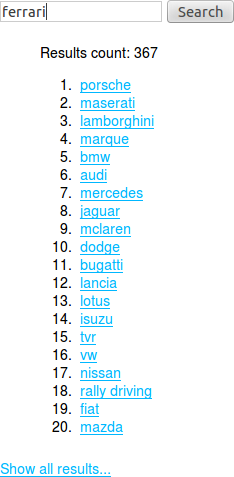
\includegraphics[height=0.6\textwidth]{figures/serelex}
        
\includegraphics[height=0.5\textwidth]{figures/spacer}
        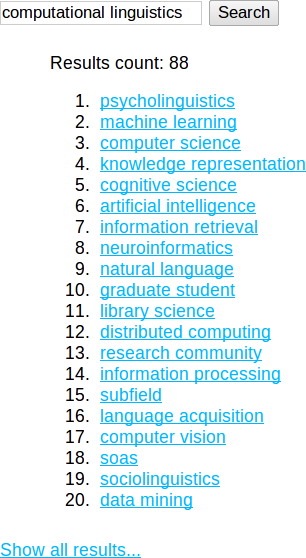
\includegraphics[height=0.6\textwidth]{figures/serelex-2}
        \end{figure}
\end{itemize}
\end{frame}







\begin{frame}
\frametitle{Lexico-syntactic patterns}

\begin{itemize}
  \item 18 patterns that extract \textbf{hypernyms}, \textbf{co-hyponyms} and \textbf{synonyms}
\begin{figure}  
    \centering
        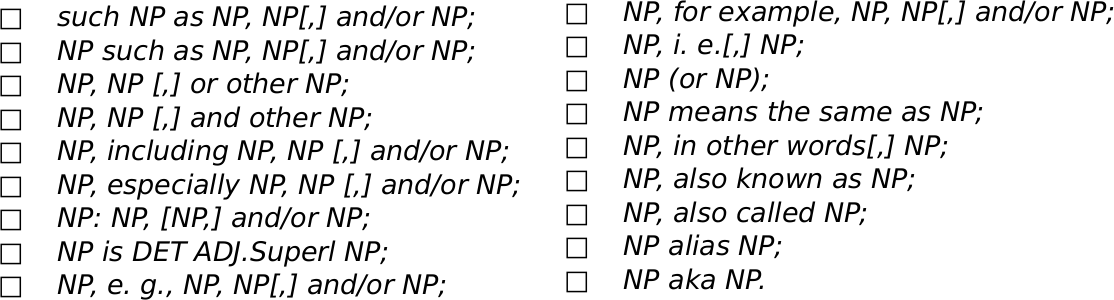
\includegraphics[width=1.0\textwidth]{figures/patterns}
    \end{figure}
\end{itemize}

\end{frame}




\begin{frame}
\frametitle{Patterns are encoded as FSTs}

\begin{itemize}
  \item Finite State Transducers (FSTs)
  \item Open source corpus processing tool \texttt{Unitex}: \url{http://igm.univ-mlv.fr/~unitex/}
  
\begin{figure}  
    \centering
        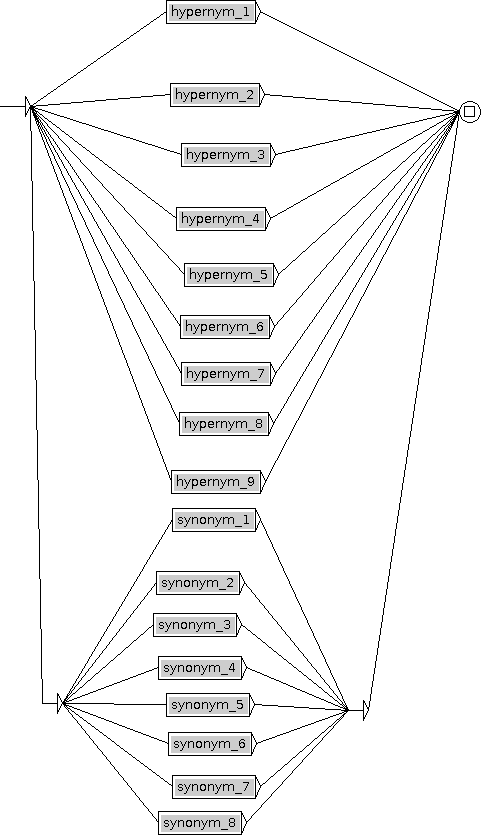
\includegraphics[width=0.3\textwidth]{figures/main-graph}
    \end{figure}
\end{itemize}

\end{frame}



\begin{frame}
\frametitle{A pattern encoded as an FST}

\begin{figure}  
    \centering
        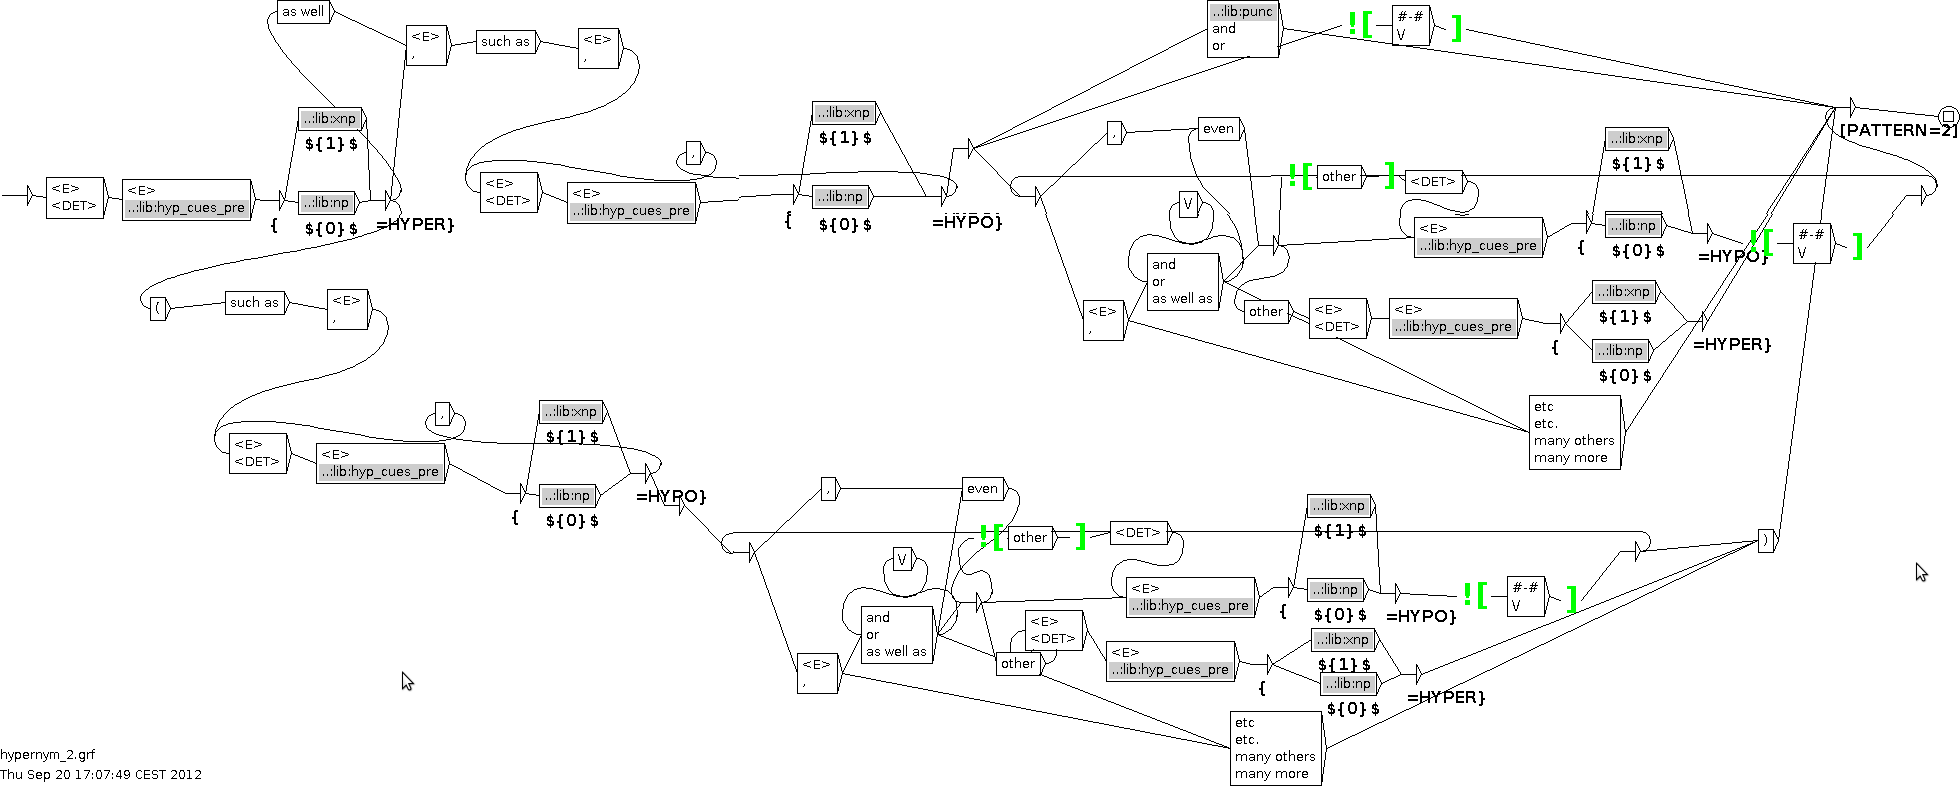
\includegraphics[width=1.0\textwidth]{figures/pattern2}
    \end{figure}

\begin{itemize}
  \item Take into account linguistic variation
  \item Unlike string-based patterns (Bollegala et al., 2007)
    
\end{itemize}

\end{frame}






\begin{frame}
\frametitle{Patterns extract concordances}

\begin{itemize}
  \item \texttt{such diverse \{[occupations]\} as
  \{[doctors]\}, \{[engineers]\} and \{[scientists]\}[PATTERN=1]}
  \item \texttt{such \{non-alcoholic [sodas]\} as \{[root beer]\} and \{[cream soda]\}[PATTERN=1]}
  \item \texttt{\{traditional[food]\}, such as \{[sandwich]\},\{[burger]\}, and \{[fry]\}[PATTERN=2]}
\end{itemize}

\end{frame}






\begin{frame}
\frametitle{Corpus}

\textbf{Corpus} Wikipedia+ukWaC: $2.9\cdot10^{12}$ tokens

\begin{figure}  
\centering
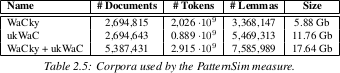
\includegraphics[width=0.7\textwidth]{figures/patternsim-table}
\end{figure}


\textbf{Extracted concordances}

\begin{itemize}
  \item Wikipedia -- 1.196.468 
  \item ukWaC -- 2.227.025 
  \item WaCypedia+ukWaC -- 3.423.493
\end{itemize}

\end{frame}





\begin{frame}
\frametitle{PatternSim Semantic Similarity}

  
$$s_{ij} = \sqrt{p_{ij}} \cdot \frac{2\cdot\mu_b }{b_{i*}+b_{*j}} \cdot \frac{P(c_i,c_j)}{P(c_i)P(c_j)}.$$


\begin{itemize}

%\item $s_{ij}$ -- semantic similarity between terms $c_i, c_j \in C$

\item $P(c_i,c_j)=\frac{e_{ij}}{\sum_{ij}e_{ij}}$ -- extraction probability of the pair $\langle c_i,c_j \rangle$, $e_{ij}$ --  frequency of co-occurrence of $c_i$ and $c_j$ in concordances $K$ 

\item $P(c_i)= \frac{f_i}{\sum_i f_i}$ -- probability of the term $c_i$, $f_i$ -- frequency of $c_i$ 
\item $b_{i*} = \sum_{j:e_{ij} \geq \beta} 1$ -- the number of extractions for term $c_i$ with the frequency $\geq \beta$, $\mu_b = \frac{1}{|C|}\sum_{i=1}^{|C|} b_{i*}$ -- the average number of extractions per term

\item $p_{ij} \in [1;18]$ -- number of distinct patterns which extracted the relation $\langle c_i, c_j \rangle$
  
 
\end{itemize}

\end{frame}




%\begin{frame}
%\frametitle{Semantic Relation Ranking}
%\begin{figure}	
%\centering
%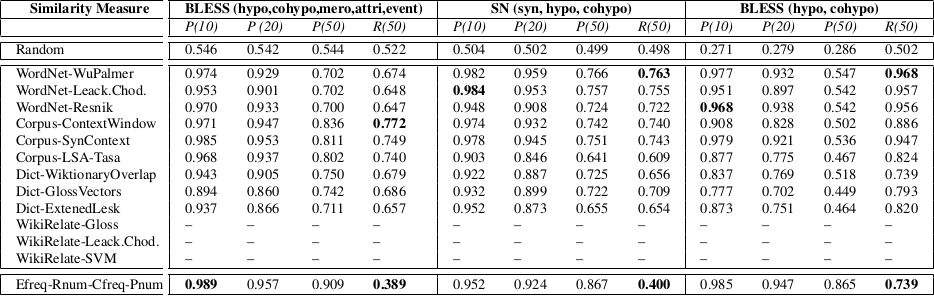
\includegraphics[width=1.0\textwidth]{figures/res-relations-mlg}
%\end{figure}
%\end{frame}




\begin{frame}
\frametitle{Semantic Relation Ranking}

\begin{itemize}
  \item Precision is \textbf{comparable or better} w.r.t. the baselines;
  \item Recall is \textbf{lower} w.r.t. the baselines.
\end{itemize}

\begin{figure}	
	\centering
	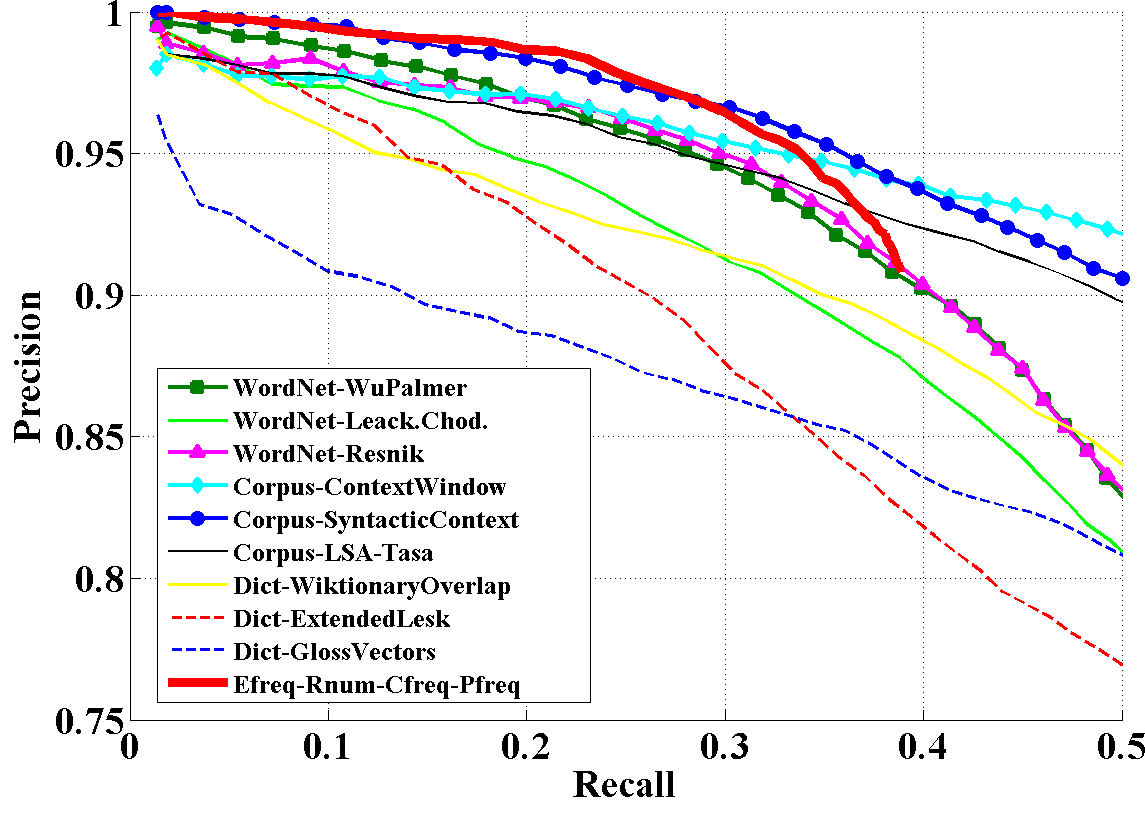
\includegraphics[width=0.65\textwidth]{figures/pr2-mlg}
	\caption{Precision-Recall graphs (the BLESS dataset).
	}
\end{figure}

\end{frame}





\begin{frame}
\frametitle{Semantic Relation Extraction}
  \begin{columns}[T]
    \begin{column}{.4\textwidth}
     
% Your text here
\includegraphics[width=0.85\textwidth]{./../figures/eval3}
    
    \end{column}
    \begin{column}{.6\textwidth}
    %\begin{block}{Your image}
\begin{itemize}
  %\item 49 words, three binary annotations;
  \item $Precision@1 \approx 0.80$;
  \item ``Good'' coverage:
  
\end{itemize}

\begin{figure}
\includegraphics[width=0.95\textwidth]{./../figures/wordnet-vs-serelex}
\end{figure}
      
    \end{column}
  \end{columns}
\end{frame}






%
%
%\section[Comparison]{Comparison of 
%Similarity Measures} 
%\subsection{  }
%
%
%
%
%\begin{frame}
%\frametitle{Related publications}
%
%\begin{itemize}
%
%\item Panchenko A. \textbf{A Study of Heterogeneous Similarity Measures for Semantic Relation Extraction.} // In JEP-TALN-RECITAL 2012 — Grenoble (France), 2012.
%
%\item Panchenko A., \textbf{Similarity Measures for Semantic Relation Extraction.} PhD thesis. Universit\'{e} catholique de Louvain. 197
%pages, 2013: \alert{Chapters 2.1, 3.1}. 
%
%\end{itemize}
% 
%\end{frame}
%
%
%
%
%\begin{frame}
%\frametitle{Compared Semantic Similarity Measures}
%
%\begin{figure}
%\includegraphics[width=1.0\textwidth]{./../figures/measures-classification}
%\end{figure}
%
%\begin{itemize}
%  \item 37 distinct measures;
%  \item \alert{Q1}: Are the measures are complementary?
%  \item \alert{Q2}: If yes, in which respects?
%\end{itemize}
% 
%\end{frame}
%
%
%
%
%
%
%
%
%
%\begin{frame}
%\frametitle{The Best Single Measures (MC, RG, WordSim, BLESS, SN)}
%
%\begin{figure}
%\includegraphics[width=1.07\textwidth]{./../figures/best}
%
%\end{figure}
%
%\begin{itemize}
%  \item Each one extracts many \alert{co-hyponyms}, e.g.: 
%  \begin{itemize}
%  \item $\langle Canon, Nikon \rangle$,
%  \item $\langle Lamborghini, Ferrari \rangle$,
%  \item $\langle Obama, Romney \rangle$.
%\end{itemize}
%\end{itemize}
%   
%\end{frame}
%
%
%
%\begin{frame}
%\frametitle{Further Results}
%
%\begin{columns}[T]
%
%\begin{column}{.6\textwidth}
%  
%\begin{block}{Most dissimilar measures}
%\begin{figure}
%\centering
%\includegraphics[width=1.0\textwidth]{./../figures/papers/7/figures/clusters-gray-2}   
%\caption{21 measures grouped according to their relation distributions. }
%\end{figure}
%\end{block}
%\end{column}
%
%\begin{column}{.4\textwidth}
%\begin{block}{Measures are  complementary w.r.t.:}
%\begin{itemize}
%  \item lexical coverage;
%  \item performances;
%  \item types of semantic relations they extract. 
%\end{itemize}
%\end{block}   
%\end{column}
%
%\end{columns}
%
%\end{frame}
%



%%%%%%%%%%%%%%%%%%%%%%%%%%%%%%%%%%%%%%%%%%%%%%%%%
\section[Hybrid Measures]{Hybrid Semantic Similarity Measure}

\subsection{}

\begin{frame}
\frametitle{Hybrid vs Single Measures}

\begin{figure}
\centering
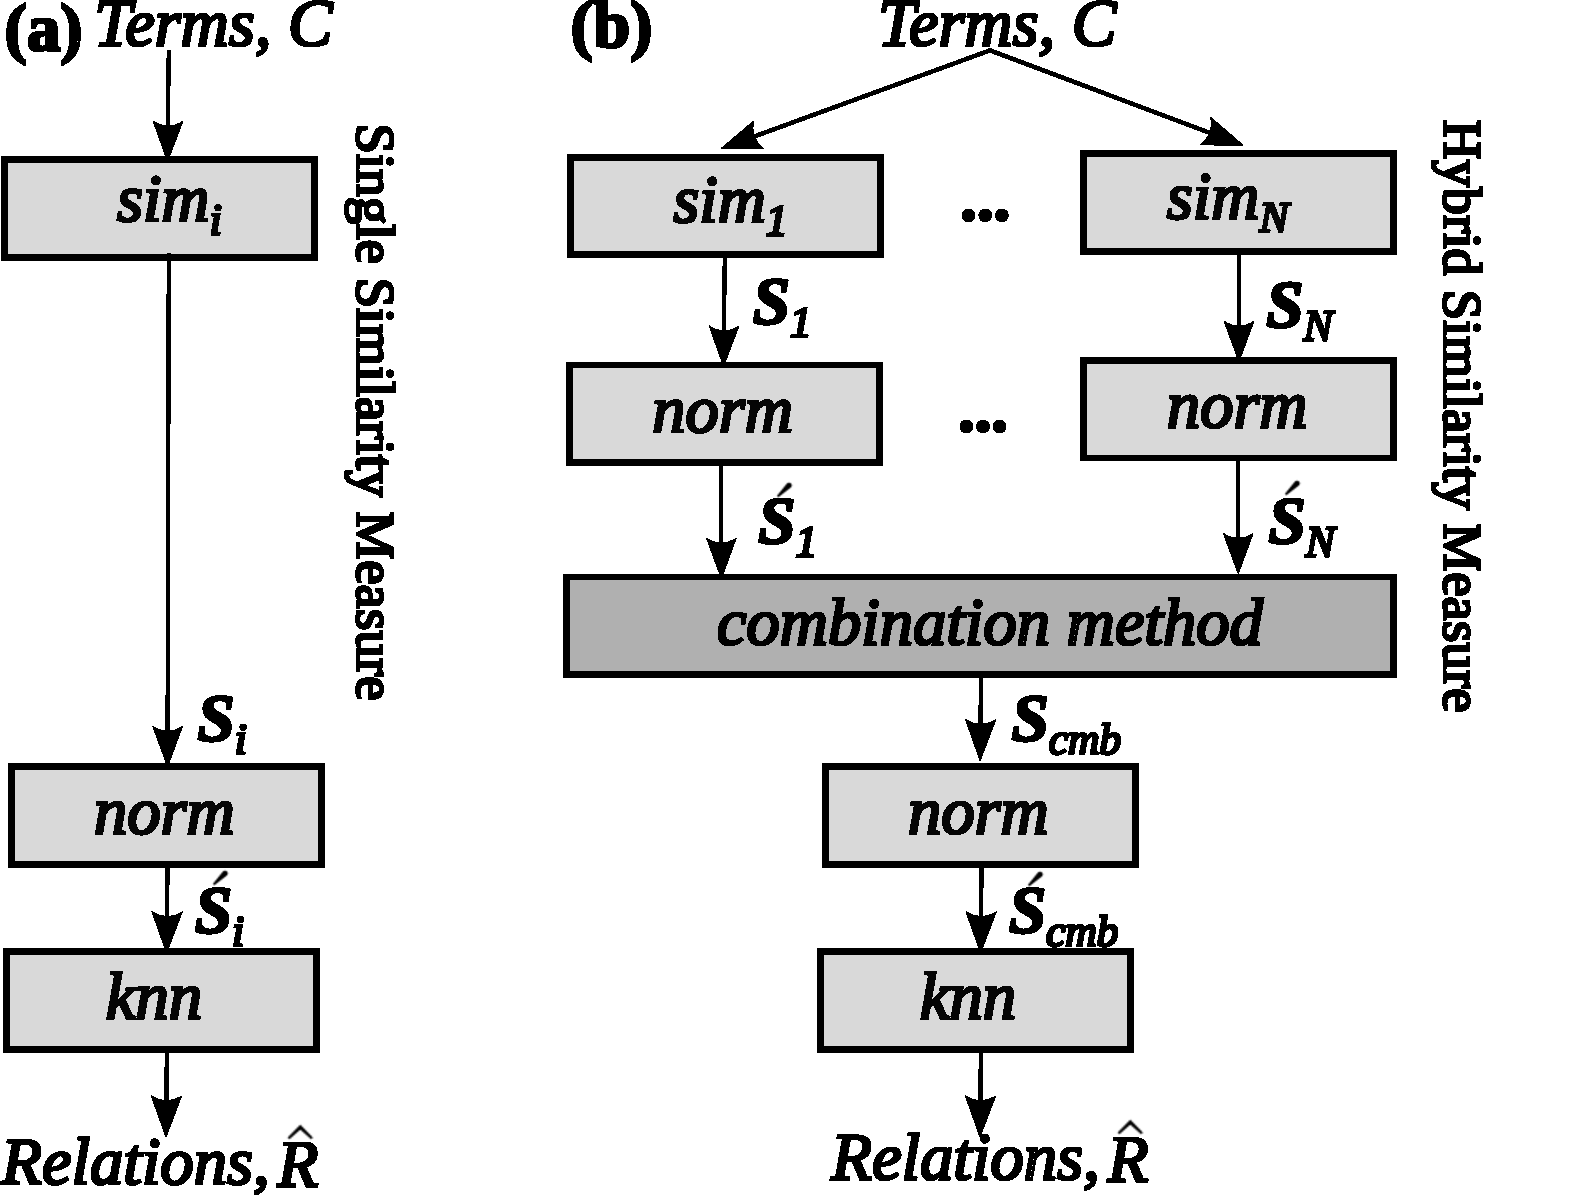
\includegraphics[width=0.65\textwidth]{./../figures/papers/4/src/figures/single-and-hybrid-2}
\caption{ Semantic relation extractor based on:
\begin{itemize}
\item \textbf{(a)} a \alert{single} similarity measure;
\item \textbf{(b)} a \alert{hybrid} similarity measure. 
\end{itemize}}
\end{figure}
\end{frame}





\begin{frame}
\frametitle{16 Features = 16 Single Similarity Measures}

	\begin{itemize}
	
	\item 5 \textbf{network-based} measures :
	\begin{enumerate}
	  \item WuPalmer;
	  \item Leacock and Chodorow;
	  \item Resnik;
	  \item Jiang and Conrath;
	  \item Lin.
	\end{enumerate} 
	\item 3 \textbf{web-based} measures (NGD-Yahoo/Bing/Google); 
		
	\item 5 \textbf{corpus-based} measures: 
	\begin{itemize}
	  \item 2 distributional (BDA, SDA)
	  \item 1 lexico-syntactic patterns (PatternSim)
	  \item 2 other co-occurence based (LSA, NGD-Factiva)
	\end{itemize}
	
	\item 3 \textbf{definition-based} measures
	\begin{enumerate}
	  \item ExtendedLesk;
	  \item GlossVectors;
	  \item DefVectors-WktWiki.
	\end{enumerate}
	 
\end{itemize}

\end{frame}




\begin{frame}
\frametitle{Implementation of the baseline measures}

\begin{itemize}
  \item \textbf{Semantic Vectors:} \url{https://code.google.com/p/semanticvectors/}
  \item \textbf{S-Space Package:} \url{https://code.google.com/p/airhead-research/}
  \item \textbf{WordNet::Similarity:} \url{http://wn-similarity.sourceforge.net}
  \item \textbf{NLTK:} \url{http://nltk.googlecode.com/svn/trunk/doc/howto/wordnet.html}
  \item \textbf{WikiRelate!}
  \item \textbf{PatternSim:} \url{http://serelex.org}
  \item \textbf{Web-based metrics:} \url{http://cwl-projects.cogsci.rpi.edu/msr}
  \item \textbf{LSA:} \url{http://lsa.colorado.edu}
  %\item \textbf{DefVectors:} \url{http://github.com/jgc128/defvectors}
\end{itemize}

\end{frame}






\begin{frame}
\frametitle{Supervised Combination of Measures}

\begin{enumerate}
  \setcounter{enumi}{7}
\item \textbf{Logistic Regression} 

\begin{itemize}
  \item  A binary \textbf{logistic regression};

\item \textbf{Positive examples} -- synonyms,
hyponyms, co-hyponyms;
\item \textbf{Negative examples} -- random relations;

  \item A relation $\langle c_i,t, c_j \rangle \in R$ is represented with a \textbf{vector of pairwise similarities}: $\mathbf{x} = (s_{ij}^1,\ldots,s_{ij}^N), N=\overline{2,16}$; 

\item Category $y_{ij}$:
$$
y_{ij} = \left\{ 
  \begin{array}{l l}
    0 & \quad  \text{ if } \langle c_i,t, c_j \rangle \text{ is a random relation} 
    \\
    1 & \quad  \text{ otherwise }\\
  \end{array} \right
  .
$$

\item \textbf{Using the model} $(w_1,\ldots,w_K)$ for combination: 
$$s^{cmb}_{ij} = \frac{1}{1 + e^{-z}}, z = \sum_{k=1}^K w_k s^k_{ij} + w_0.$$

\end{itemize}
\end{enumerate}

\end{frame}



\begin{frame}
\frametitle{Supervised Combination Methods}

\begin{enumerate}
  \setcounter{enumi}{8}
\item \textbf{SVM}. 


\begin{columns}
  \begin{column}{0.5\textwidth}
\begin{figure}
\centering
\includegraphics[width=1.0\textwidth]{./../figures/svm}
%\caption{SVM: maximal margin hyperplane. }
\end{figure}
    
  \end{column}

  \begin{column}{0.5\textwidth}
\begin{itemize}
\item The weights $\mathbf{w}$ and the support vectors $SV$: 

$$
\mathbf{w} = \sum_{x_i \in SV} \alpha_i y_i \mathbf{x}_i.  
$$

\item \textbf{Using the model} 

$$
s_{ij}^{cmb} = \mathbf{w}^T\mathbf{x} + b = \sum_{k=1}^K w_i s_{ij}^k + b.
$$

\end{itemize}    
  \end{column}
\end{columns}





\end{enumerate}

\end{frame}






\begin{frame}
\frametitle{Hybrid Similarity Measures}
\begin{figure}
\centering
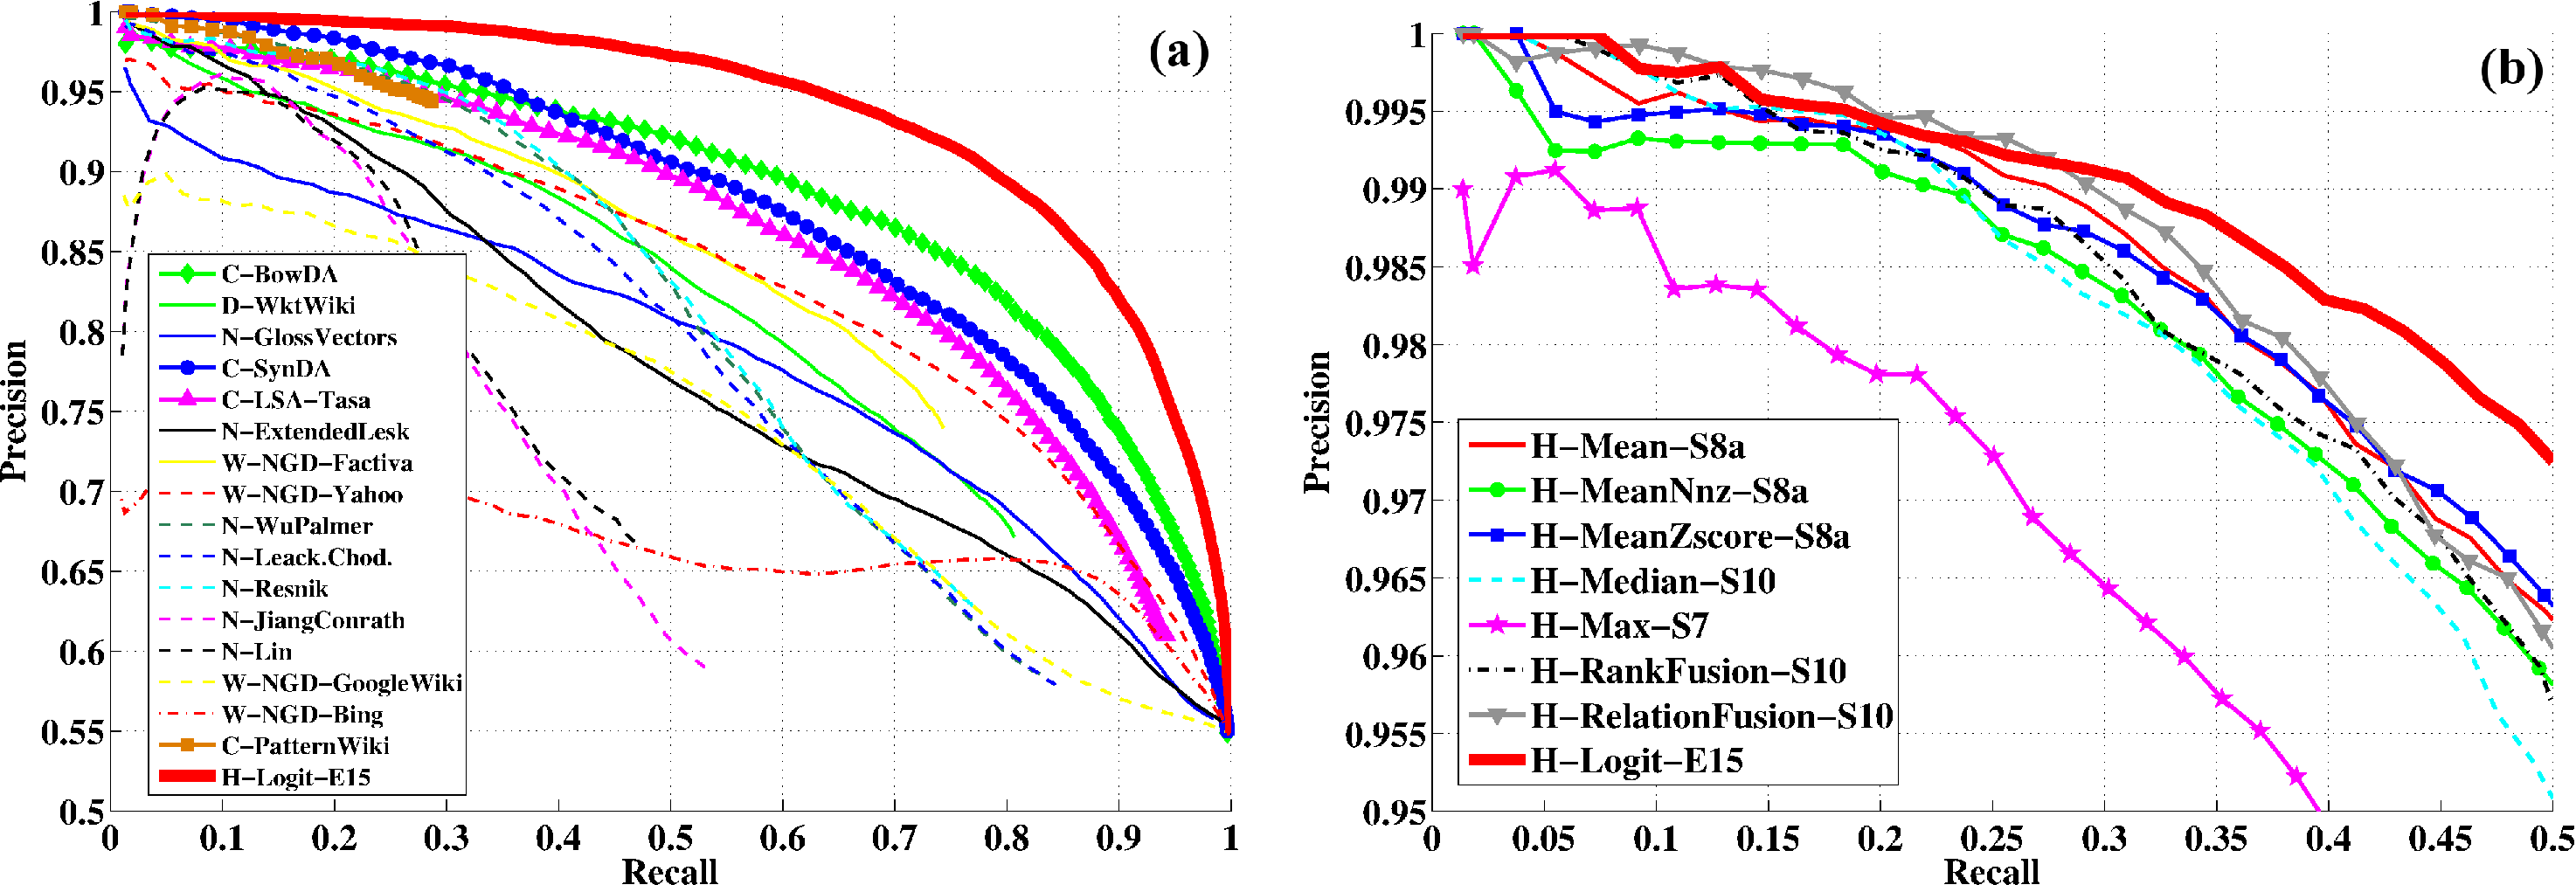
\includegraphics[width=1.0\textwidth]{figures/pr}
%\caption{

%}
\end{figure}

Precision-Recall graphs calculated on the BLESS dataset:
\begin{itemize}
  \item \textbf{(a)} 16 single measures and the best hybrid measure Logit-E15;
  \item \textbf{(b)} 8 hybrid measures.
\end{itemize}

\end{frame}



\begin{frame}
\frametitle{Supervised Hybrid Similarity Measures}
\begin{figure}
\centering
\includegraphics[height=0.4\textwidth]{./../figures/sn-accuracy}
\includegraphics[height=0.4\textwidth]{./../figures/bless-accuracy}
%
\includegraphics[height=0.025\textwidth]{./../figures/spacer}
%\includegraphics[height=0.36\textwidth]{./../figures/bless-precision10}
%\includegraphics[height=0.36\textwidth]{./../figures/bless-precision20}
%
\includegraphics[height=0.025\textwidth]{./../figures/spacer}
%\includegraphics[height=0.36\textwidth]{figures/bless-precision50}
%\includegraphics[height=0.36\textwidth]{figures/bless-recall50}     
     
\caption{ Meta-parameter optimization with the grid search of the C-SVM-radial-E15 measure.  }
\label{fig:radial-optimization}
\end{figure}
\end{frame}



\section[Word Embeddings]{Word Embeddings}

\begin{frame}
\frametitle{Key facts}

\textbf{Word embedding} is a dense vector representing a word obtained during a training of a neural network on a big corpus. 

\begin{itemize}
\item Semantic similarity is cosine of word embeddings. 

\item The training process is known as representation learning. 

\item Learning methods rely on distributional hypothesis of Harris (1954), similarly to classical distributional models. 

\item Most popular representation learning methods: 

\begin{itemize}
\item Continuous Bag of Words (CBOW) 

\item Skip-Gram Model 

\item Global Vectors of for Word Representation (GloVe)
\end{itemize}
\end{itemize}

\end{frame}



\begin{frame}
\frametitle{Distributional Hypothesis: "You shall know the word by the company it keeps" (Firth, 1957)}

\begin{figure}
\centering
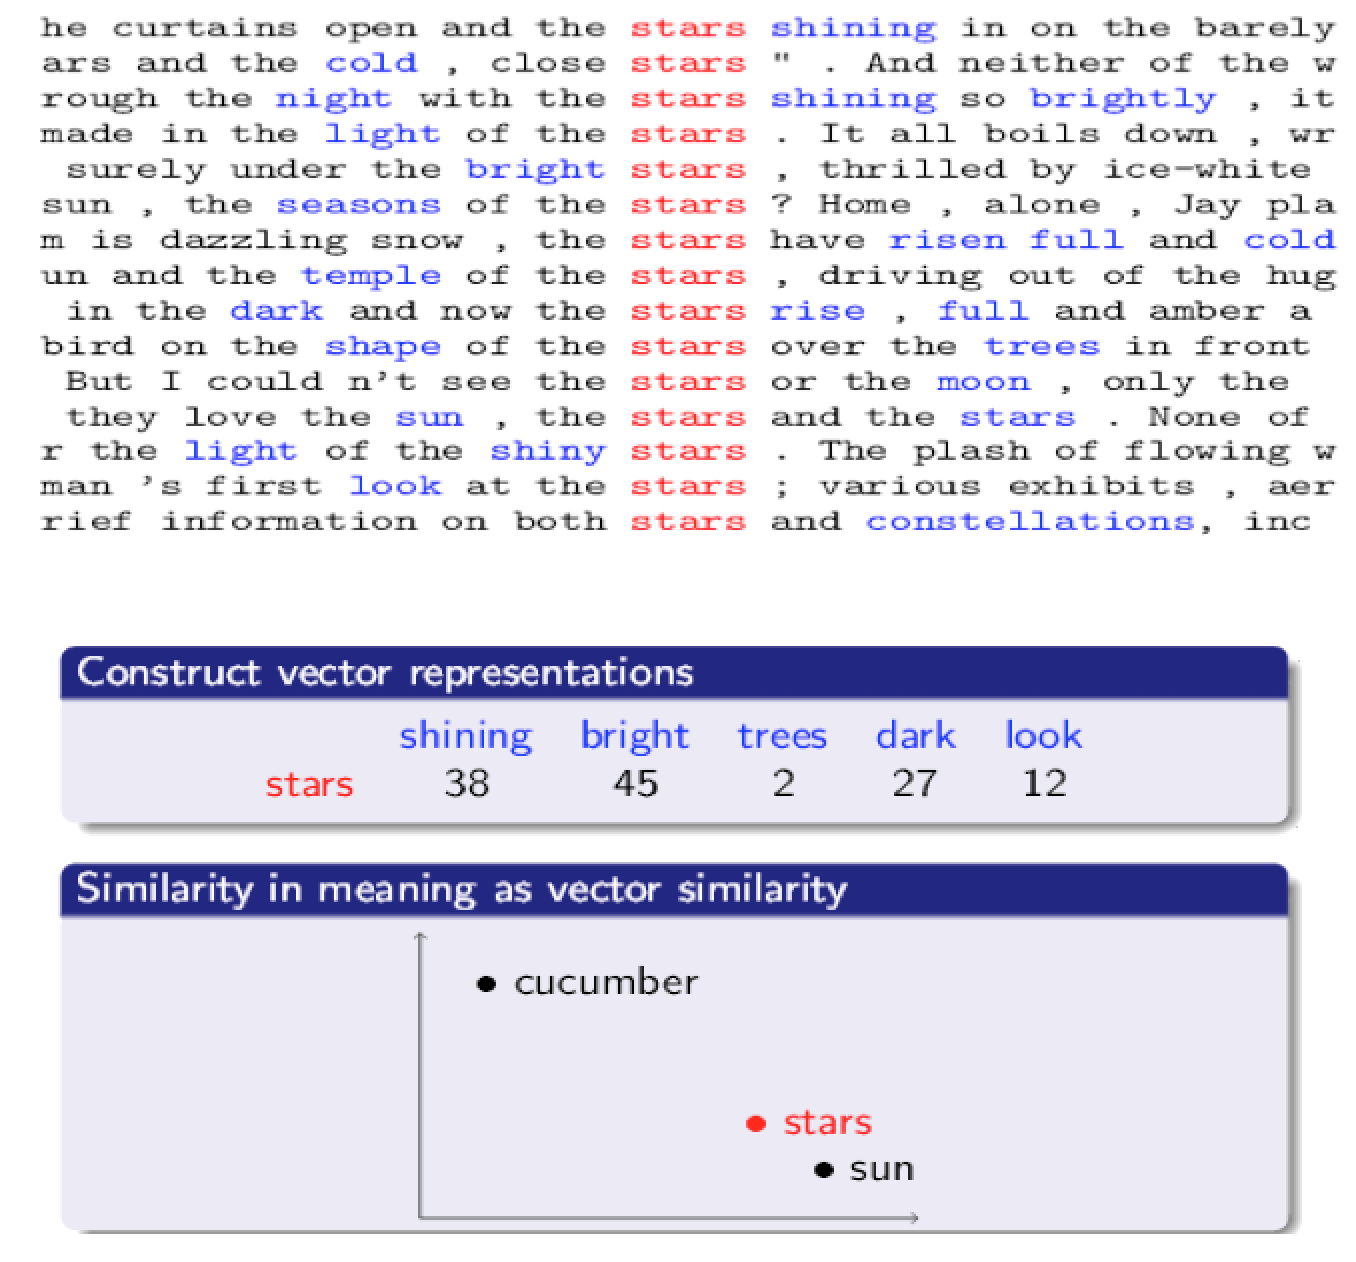
\includegraphics[height=0.91\textwidth]{./../grefenstette}
\end{figure}
	
\end{frame}




\begin{frame}

\frametitle{Skip-Gram Model}

\begin{itemize}

\item Probability that word $w$ appears in some context $c$:
{\small
$$ P(D=1| w,c;\theta) = \frac{1}{1+ \exp^{-V_c W_w}}$$  
}

\item Assign high probability to $(c,w$) pairs which appear in texts ($corp$) and low probability to the ones which cannot ($rand$): 
{\small 
$$\theta^* = arg max \prod_{(c,w) \in corp} P(D=1|w,c;\theta) \prod_{(c,w) \in rand} (1 - P(D=1|w,c;\theta))$$ 
}
\item $\theta = (V,W)$ are two matrices with columns $V_c$ and $W_w$ contain vectors of $dim$ dimensions of the context $c$ and the word $w$. 

\item The "embedding" of the word $w$ is the vector $W_w$. 


	
\end{itemize}

	
\end{frame}



\begin{frame}
\frametitle{Shared Task on Russian Semantic Similarity}

\begin{figure}  
    
\includegraphics[width=0.3\textwidth]{./../dialog_logo_en}
\end{figure}

\begin{itemize}
\item \url{www.dialog-21.ru/en/evaluation/2015/semantic}

\item  \textbf{Relatedness track}: Synonyms, Hypernyms, Human Judgements about Semantic Similarity
\item  \textbf{Associative track}: Free associations 
\end{itemize}

\end{frame}




\begin{frame}
\frametitle{ Evaluation }

\begin{figure}  
    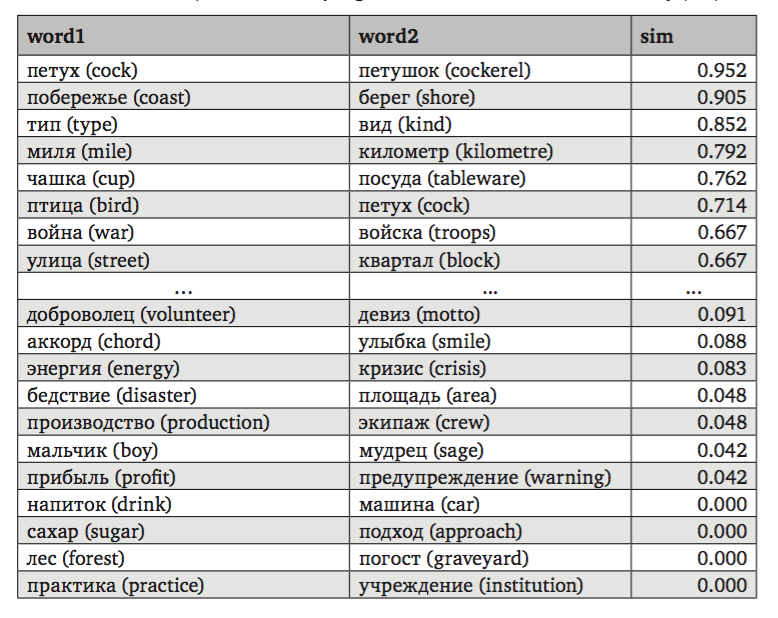
\includegraphics[width=0.8\textwidth]{../russe-evaluation}
\end{figure}

\end{frame}





\begin{frame}
\frametitle{ Best Systems }

\begin{figure}  
    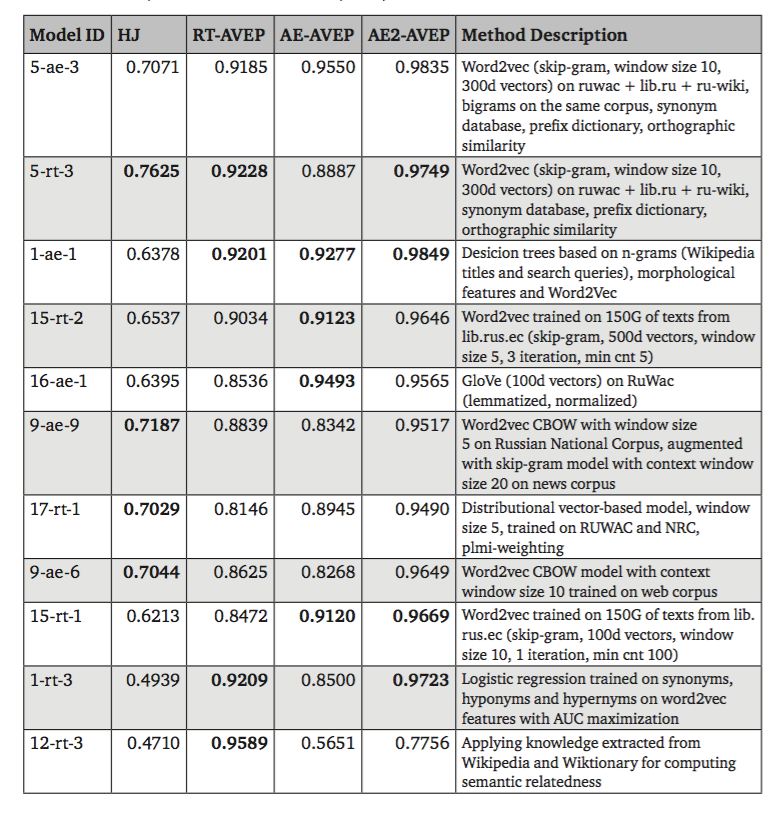
\includegraphics[width=0.65\textwidth]{../russe-results}
\end{figure}

\end{frame}


\begin{frame}
\frametitle{Skip-Gram on 150Gb of   lib.rus.ec corpus}
\begin{figure}
\centering
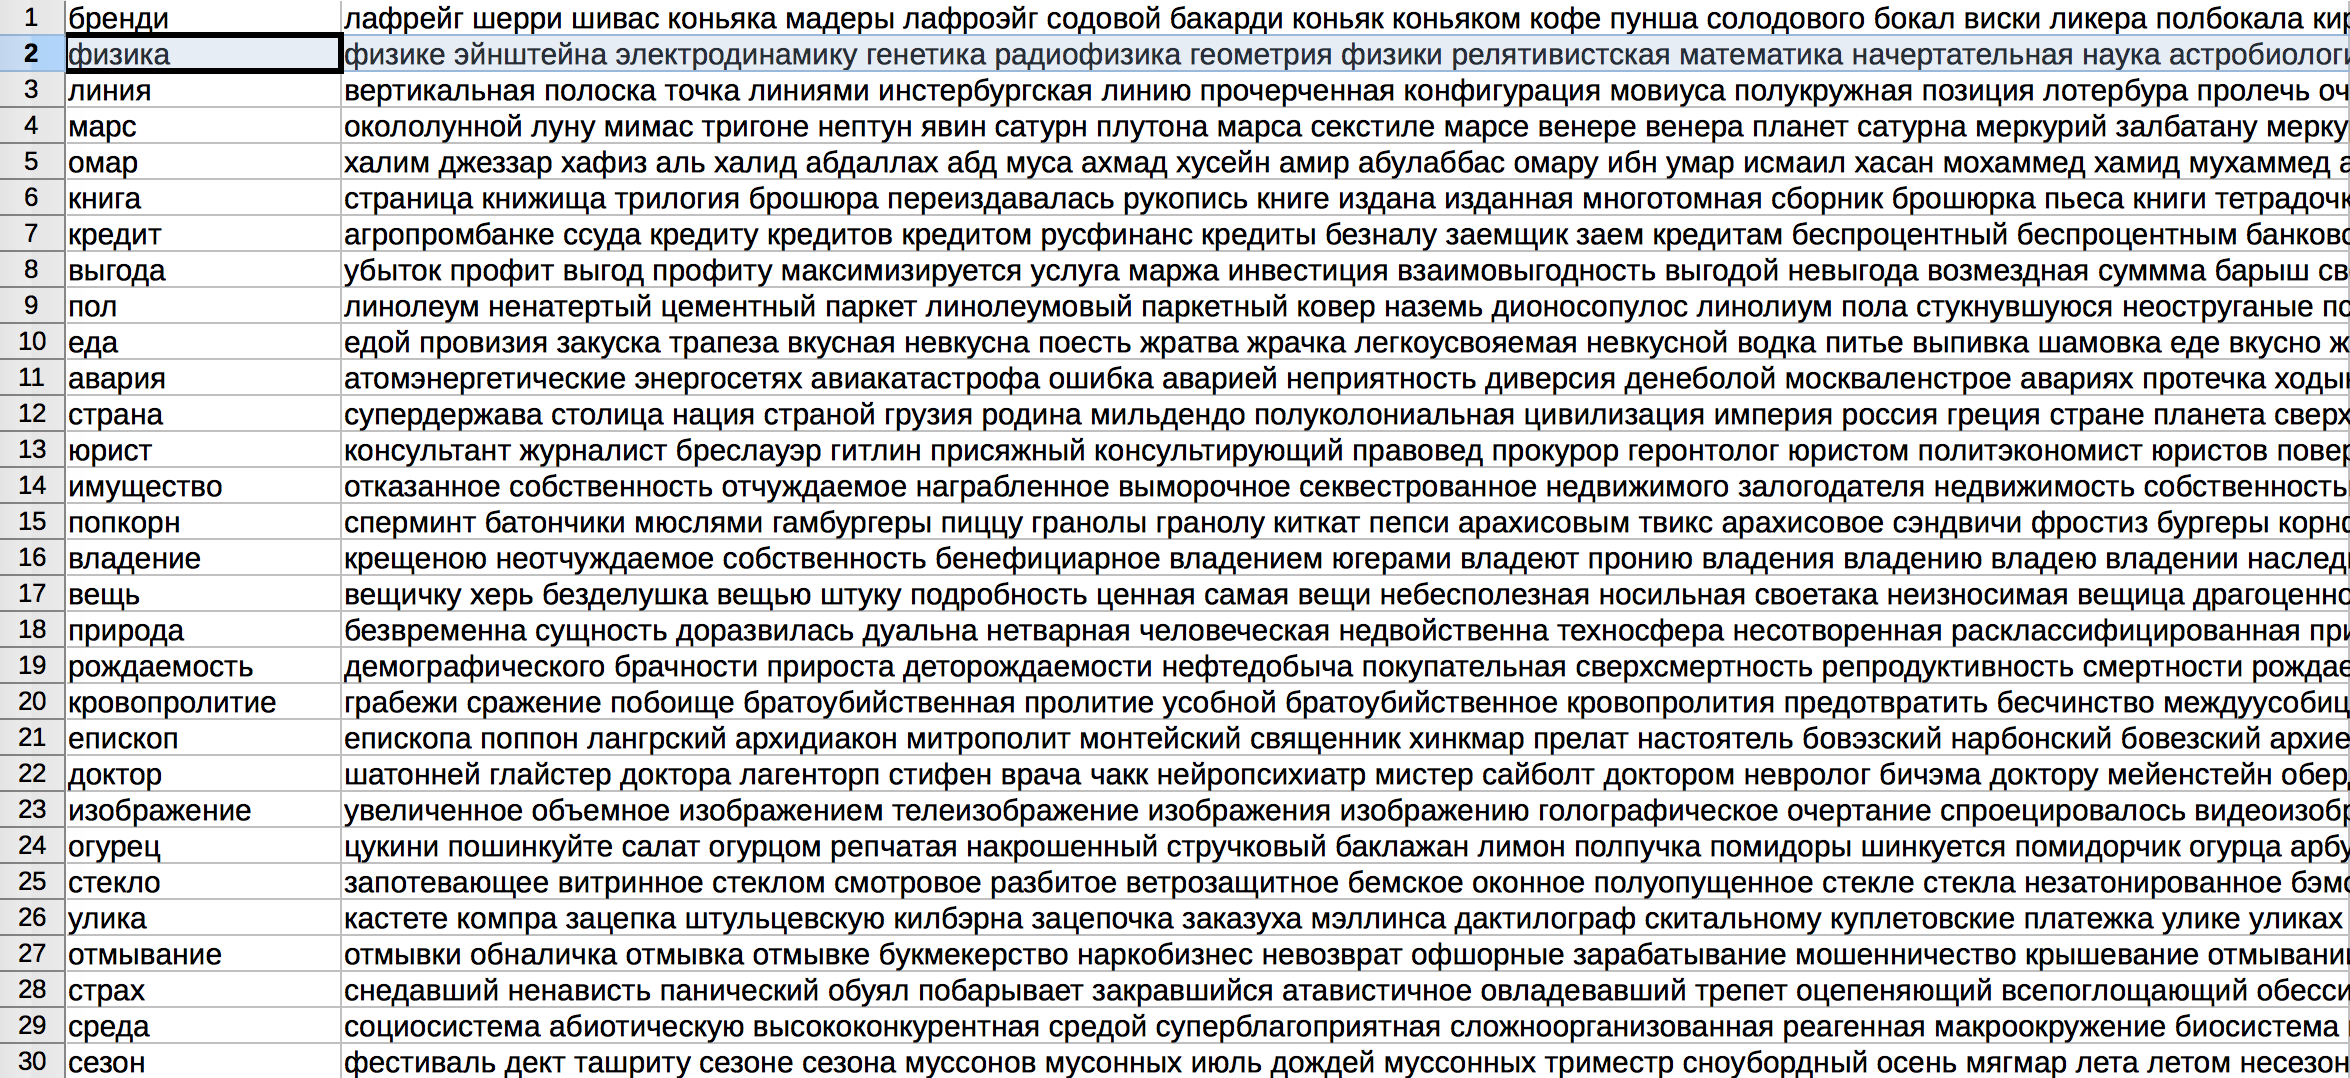
\includegraphics[width=1.0\textwidth]{./../dt-rus}
\end{figure}
	
\end{frame}



%
%
%\begin{frame}
%\frametitle{ Results: Semantic Relation Classification, Associations }
%
%\begin{figure}  
%    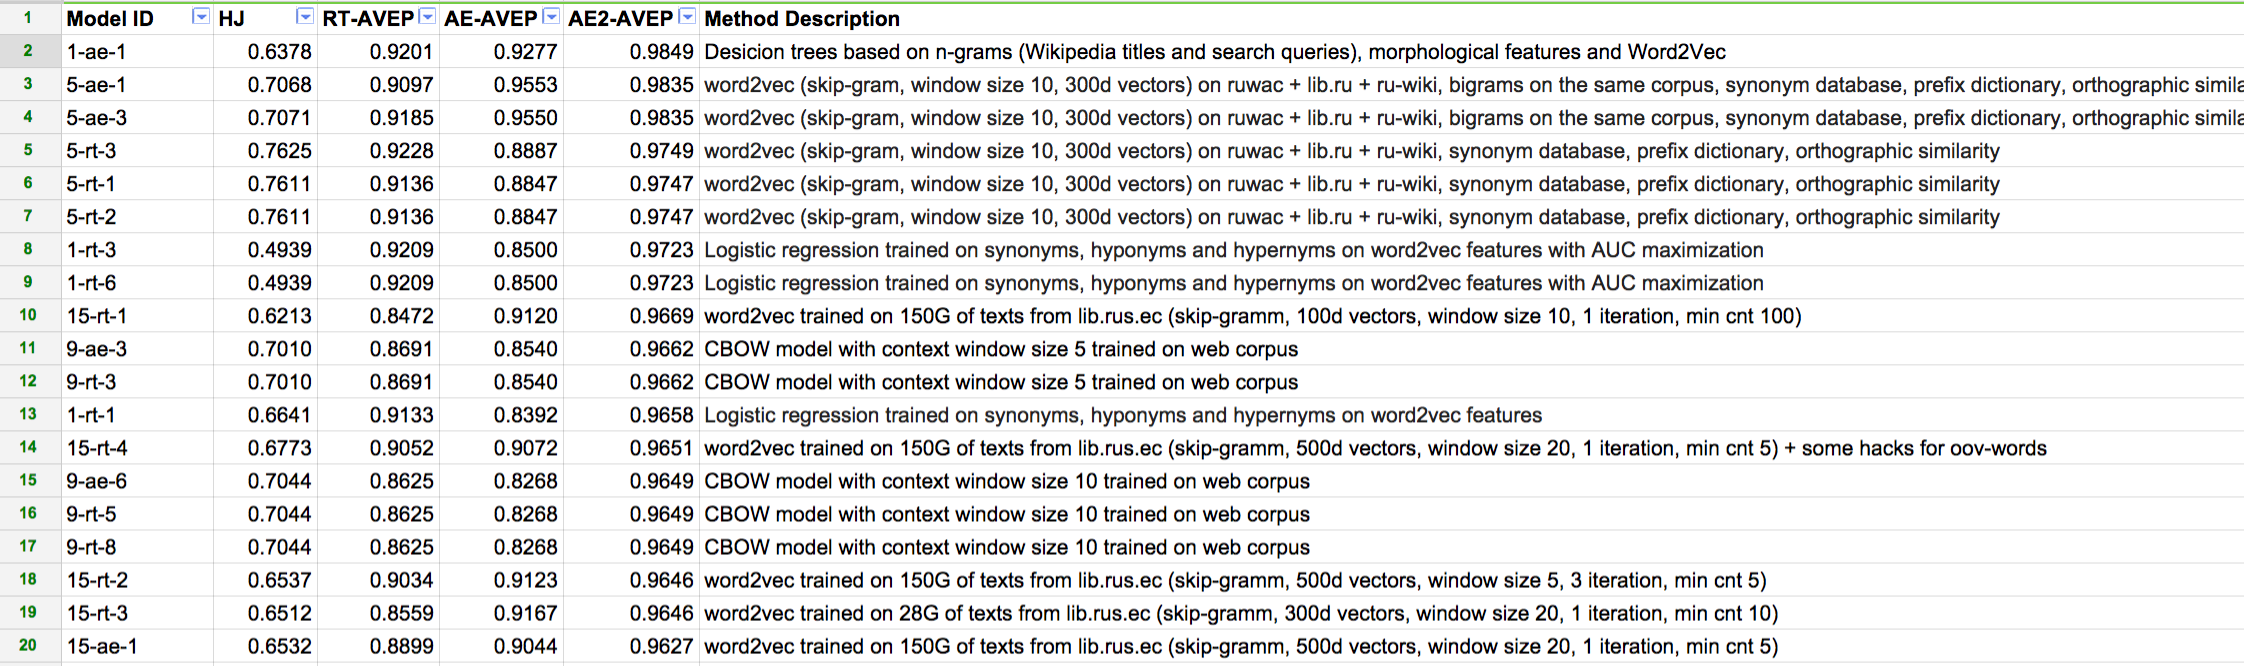
\includegraphics[width=1.45\textwidth]{figures/results-ae2}
%\end{figure}
%
%\end{frame}


